%!TEX root = ../dokumentation.tex

\chapter{Materialien und Methoden} \label{ch:materialsAndMethods}

% -   Politikapparat und Parteienlandschaft
% -   Erörterung, welche Medienplattformen und Nachrichtenquellen verwendet werden sollen
% -   Auswahl von Quellen und Sammeln von Daten
% -   NLP-Pipeline
% -   Machine Learning / Clustering

% \subsection{Check-worthy sentence detection}

% % TODO: Check if this is even relevant for this paper 

% % \begin{figure}[H]
% %     \centering
% %     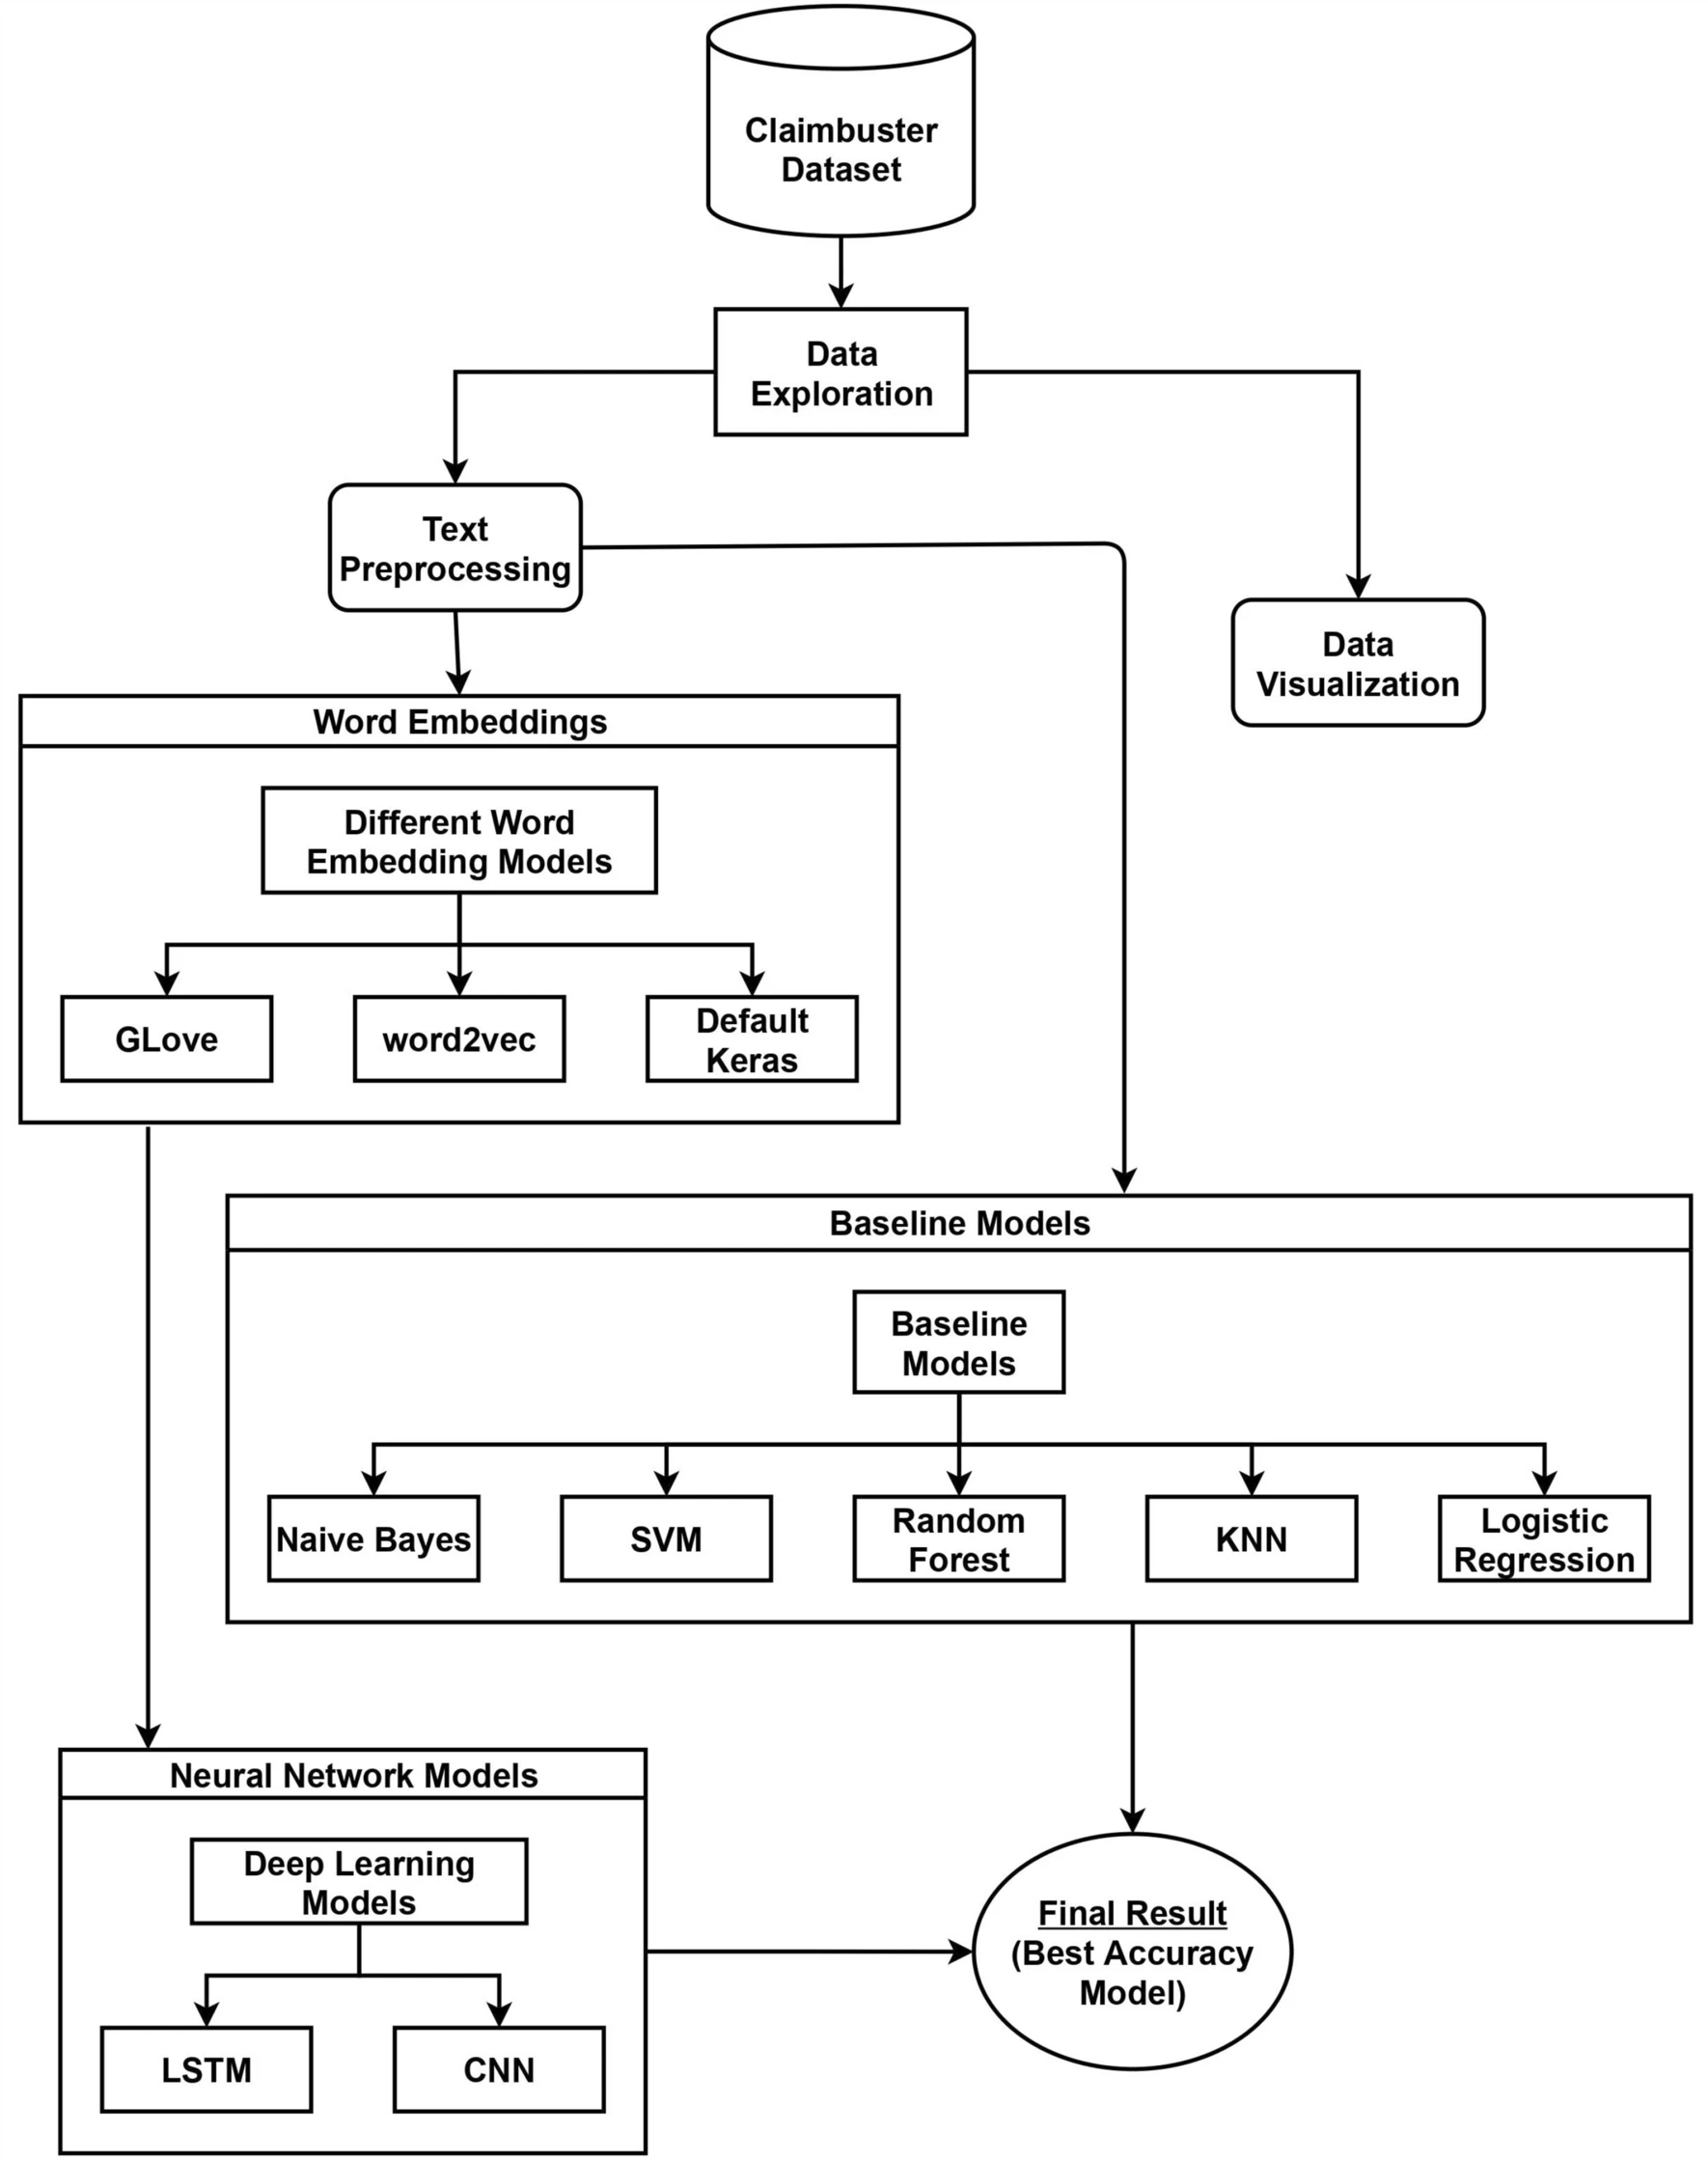
\includegraphics[width=0.8\textwidth]{images/workflow_of_experiment_design.png}
% %     \caption[Workflow of Experiment Design]{Workflow of Experiment Design \autocite{jha_towards_2023}} \label{fig:workflowExperimentDesign}
% % \end{figure}

% Das G2CW Framework von \textcite{jha_towards_2023} ermöglicht es zu prüfen, ob ein englischer Satz einen Fakt enthält. Zusätzlich klassifiziert das Modell, ob dieser Fakt irrelevant ist, oder ob es sich lohnt, die Richtigkeit des Satzes zu überprüfen (F1-Score \num{0.92}).

% Für das Training des \ac{ML} Modells werden zwei unterschiedliche Arten von Modellen trainiert. Als Ausgangsmetrik werden herkömmliche Modelle wie Naive Bayes, \ac{SVM} und Random Forest verwendet. Diese werden mit Features aus einzelnen Sätzen und \ac{POS} Features trainiert. Zusätzlich werden Deep Leaarning Modelle wie \ac{LSTM} und \ac{CNN} verwendet. Für das Training von den letzten Modellen verwenden \textcite{jha_towards_2023} Word Embedding Modelle wie GLove, word2vec und Keras.

\section{Deutsche Politik in der 19. Legislaturperiode}

Eine gute Übersicht über die notwendigen politikwissenschaftlichen Hintergründe bieten \textcite{bukow_innerparteiliche_2013}, die die Organisation und Funktion der deutschen Parteien beschreiben.

\subsection{Heterogenität der Parteienlandschaft}

Lorem Ipsum

\begin{figure}[H]
    \centering
    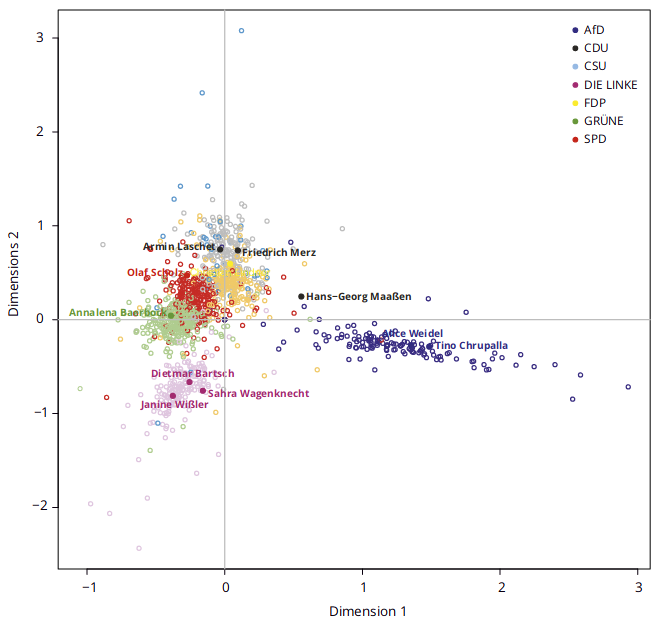
\includegraphics[width=0.5\textwidth]{data/images/positionierung_ausgewaehlter_kandidaten.png}
    \caption[Positionierung ausgewählter Kandidat:innen]{Positionierung ausgewählter Kandidat:innen innerhalb eines zweidimensionalen politischen Raums \autocite{saltzer_bundestagswahl_2022}} \label{fig:positionierungAusgewaehlterKanidaten}
\end{figure}

\subsection{Politische Ereignisse im Untersuchungszeitraum}

\subsubsection{Durchgeführte Wahlen}

\subsubsection{Besondere Vorkommnisse} 

% TODO: besseren Titel überlegen

\subsection{Themenschwerpunkte in Debatten}

% TODO: Remove reference

\ac{MdB}

% \section{NLP}

% \subsection{Cleaning Pipeline}

% - Common Sense aus der Literatur

\section{Repräsentationsformen von Text}

% TODO: Either describe specific models or the underlying architecture (e.g. fasttext or n-gram method)

Die Theorie hinter Word Embeddings wurde erstmals anhand von Wörtern, die in einem ähnlichen Kontext auftreten, festgestellt, da diese häufig auch eine ähnliche Bedeutung besitzen (z. B. Augenarzt und Optiker) \autocite[103]{jurafsky_speech_2023}.

Nach \textcite[103]{jurafsky_speech_2023} unterscheiden sich Embeddings in statische und kontextbasierte Word Embeddings.

Herkömmliche Methoden wie \ac{BoW} und \ac{TF-IDF} generieren unkomprimierte Vektoren und skalieren linear mit der Anzahl an einzigartigen Wörtern. Ein alternativer Ansatz dazu sind sogenannte Word Embeddings. Mittels dieser werden Wörter nicht mehr eins zu eins in einzelne Features encodiert, sondern mittels mehrdimensionalen Vektoren\footnote{Häufig bestehen Word Embeddings aus \num{300} Dimensionen} repräsentiert.

\subsection{\acl{BoW}}

% TODO: Check if formula is correct

\begin{itemize}
    \item \ac{BoW} führt zu Matrizen mit den Maßen \(n(\{v_i\}_{i\epsilon\{1,\dots,n\}}) \times n(rows)\) (Anzahl an einzigartigen Wörtern x Anzahl an Einträgen)
\end{itemize}

\subsection{\acl{TF-IDF}}

% TODO: Add function for dimensions

\subsection{FastText}

Lorem Ipsum

\subsection{GloVe}

% TODO: Check if Spacy uses GloVe or not

Lorem Ipsum

\subsection{ELMo}

Lorem Ipsum

\section{\acl{ML} Verfahren}

% TODO: Add and descripe models used for modeling

\subsection{BERT}

Lorem Ipsum

\subsection{LSTM}

Lorem Ipsum

\section{Zusammenfassung}
